\section{Aufgabe 1: Entscheidungsbäume}
\subsection{Feature Engineering}

\subsubsection{Analyse der Zielvariable}
Wie Abbildung \ref{fig:disc_target_variable} entnommen werden kann, ist die Ausprägung der Zielvariable ungleich auf beide Klassen verteilt. Die Klassifizierungsgenauigkeit eines Modells muss demnach unter Berücksichtigung der sogenannten \emph{Null Accuracy} bewertet werden. Unter \emph{Null Accuracy} versteht man die Genauigkeit eines Modells, dass unabhängig von allen Eingaben immer die am häufigsten auftretende Klasse vorhersagt. In unserem Fall würde ein Modell, welches immer Regen vorhersagt, eine Klassifizierungsgenauigkeit von 79,39\% erreichen. Das Ziel der nachfolgenden Schritte ist also ein Modell mit einer besseren Klassifizierungsgenauigkeit als die \emph{Null Accuracy} aufzubauen.
\begin{figure}[ht]
	\centering
	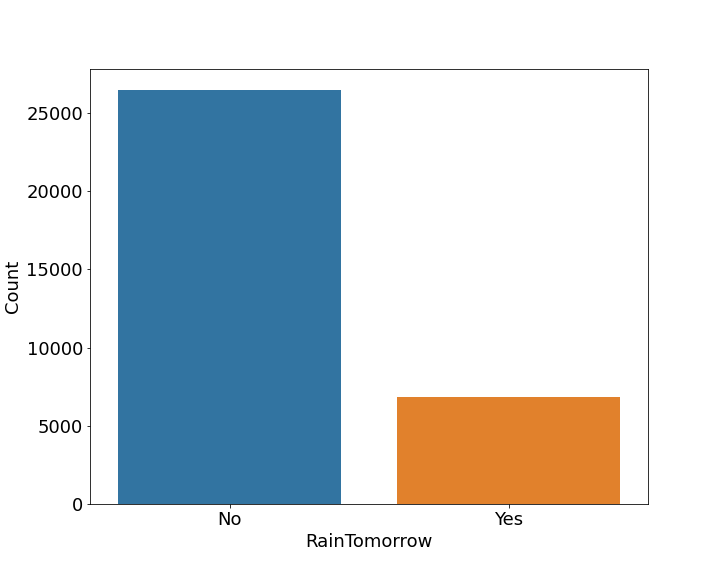
\includegraphics[width = 0.45\textwidth]{Bilder/distribution_target_variable.png}
	\caption{Verteilung der Zielvariable}
	\label{fig:disc_target_variable}
\end{figure}
\subsubsection{Fehlende Werte}
Der zu untersuchende Datensatz beinhaltet fehlende Werte. Im Folgenden werden Methoden beschrieben, wie mit den fehlenden Werte umgegangen wurde:
\begin{description}
	\item[Fehlende Zielvariable:]
	 Im ersten Schritt wurden alle Beobachtungen, welche keinen Wert für die Zielvariable \emph{RainTomorrow} aufweisen, aus dem Datensatz entfernt. Damit wurde die Anzahl an Beobachtungen um 834 auf 33402 reduziert.
	 \item[Spalten mit fehlenden Werten:]
	 In einem nächsten Schritt werden die Spalten aus dem Datensatz entfernt, in denen mehr als 40\% der beinhaltenden Variablen fehlen. Namentlich wurden somit die Spalten \emph{Evaporation, Sunshine, Cloud9am} sowie \emph{Cloud3pm} aus dem Datensatz entfernt. Der Schwellwert von 40\% wurde empirisch festgelegt und hat zu den besten Klassifizierungsergebnissen geführt.
	 \item[Beobachtungen mit fehlenden Werten]
	 Des Weiteren werden Beobachtungen aus dem Datensatz entfernt, von denen mehr als 50\% der Variablen fehlen. Durch diesem Schritt wurden 55 Beobachtungen aus dem Datensatz entfernt.
	 \item[Imputation]
	 Durch die zuvor beschriebenen Methoden ist der Datensatz immer noch  nicht frei von fehlenden Werten. Um diese zu ersetzen, werden für kategorische und numerische Variablen verschiedene Strategien zur Imputation verfolgt. Fehlende numerische Werte werden mit dem Median der jeweiligen Variable ersetzt. Der Median wurde gewählt, da dieser im Vergleich zum Mittelwert robuster gegenüber Ausreißern ist. Für kategorielle Variablen hingegen wird der am häufigsten vorkommende Wert verwendet. Wichtig bei der Ermittlung des Medians bzw. des häufigsten Wertes ist, dass dieser ausschließlich mit Hilfe der Trainingsdaten (siehe Abschnitt \ref{section:train_test_split}) ermittelt wird. Es muss davon ausgegangen werden, dass die Testdaten nicht bekannt sind. Die Ermittlung auf Basis des gesamten Datensatzes, inklusive der Testdaten, würde zu \emph{Data Leakage} führen und ist zu vermeiden. Die auf Basis der Trainingsdaten ermittelten Werte für die Imputation werden auf die Trainings- und Testdaten angewendet.
\end{description}

\subsubsection{Merkmalserstellung und Aufteilung}
Eine weit verbreitete Technik des Feature Engineerings ist die Erstellung zusätzlicher Merkmalen. Somit wurde die Variable \emph{MinMaxDiff} erstellt, welche die Differenz zwischen der minimalen und der maximalen Tages-Temperatur angibt. Des Weiteren wurden die Variablen \emph{PressureDiff, HumidityDiff und WindSpeedDiff} als Differenz der Beobachtungen am Morgen und Abend erstellt. Das Feld \emph{Datum} wurde in die Merkmale \emph{Year, Month} und \emph{Day} aufgeteilt.

\subsubsection{Diskretisierung}
%TODO: Entscheidungsbäume sind doch auch sensibel gegenüber vieler verschiedener Werte... Das wäre noch ein gutes Argument
Die Diskretisierung eines Merkmals kann eine Überanpassung bei der Erstellung von Modellen verhindern, indem der Wertebereich des Merkmals minimiert und somit generalisiert wird. Hierbei muss beachtet werden, dass der Informationsverlust durch die Diskretisierung nicht zu groß ist. Eine Diskretisierung wurde für das Merkmal \emph{Month} durchgeführt, indem es in das Merkmal \emph{Season} umgewandelt wurde. Das Merkmal \emph{Season} fasst immer 3 Monate zu einer Jahreszeit zusammen.

\subsubsection{Kodierung kategorischer Werte}
Um kategorische Werte für weitere Analysen verwenden zu können, müssen diese in numerische Werte umkodiert werden. Hierbei wurden die folgenden Strategien Angewendet:
\begin{description}
	\item[Binäre Kodierung]
	Die Zielvariable \emph{RainTomorrow}, sowie die Variable \emph{RainToday} liegen in den Ausprägungen \emph{Yes} und \emph{No} vor. Für eine weitere Verarbeitung wurden die Ausprägungen in eine numerische binäre Darstellung umgewandelt.
	\item[One-Hot-Kodierung]
	%TODO: One-Hot beschreiben?
	Das neu diskretisierte Merkmal \emph{Season} wird mittels \emph{One-Hot-Kodierung} umgewandelt. Eine \emph{Label-Kodierung}, also eine einfache Kodierung mit einem zufälligen Zahlenwert pro auftretender Variablenausprägung, hat den Nachteil, dass dadurch eine Variable entsteht, die gegebenenfalls metrisch interpretiert wird.
	\item[Ziel-Kodierung]
	Mit Hilfe der Ziel-Kodierung werden die Merkmale \emph{Location, WindGustDir, WindDir9am} und \emph{WindDir3pm} umgewandelt. Hierbei werden die Merkmalsausprägungen als ihren Einfluss auf die Zielvariable kodiert.
\end{description}

\subsubsection{Bereinigung von Ausreißern}
%TODO: Haben wirklich nur die Vairablen ausreißer?? Ich hatte nur die im code untersucht...
Ausreißer können die Performance eines Modells mindern, indem sie als Hebelwerte agieren und somit die Schätzungen der Zielvariable verzerren. Aus diesem Grund werden die Merkmale des Datensatz hinsichtlich ihrer Ausreißer begutachtet. Es wird ersichtlich, dass Merkmale wie \emph{Rainfall} und \emph{WindGustSpeed} abweichende Werte aufweisen. Das Entfernen dieser Werte aus dem Datensatz führt jedoch zu einer schlechteren Performance der im folgenden Abschnitt besprochenen Entscheidungsbäume. Deshalb werden die Beobachtungen nicht aus dem Datensatz entfernt.

\subsubsection{Normalisierung der Daten}
Für Entscheidungsbäume ist eine Normalisierung der Daten nicht Notwendig. Um das \emph{Feature Engineering} jedoch unabhängig vom gewählten Klassifizierer und auch im Hinblick auf neuronale Netze oder \emph{Support Vector Machines} (SVMs) durchzuführen, wird es an dieser Stelle durchgeführt. Die Werte der einzelnen Variablen werden dabei auf den Wertebereich $[0, 1]$ umskaliert.
 
\begin{comment}
\subsubsection{Variablenselektion}
%TODO: Brauchen wir die Variablenselektion wirklich? Oder wird das durch den Max_detph parameter vom Baum geregelt...?
Nach Abschluss der oben aufgeführten Schritte verfügt der Datensatz über 28 Einflussvariablen. Durch eine Variablenselektion soll die Anzahl dieser Einflussvariablen verringert werden. Das hat zum einen den Vorteil, dass Modelle  besser interpretierbar sind. Zum Anderen wird die Generalisierungsfähigkeit eines Modells erhöht, indem Merkmale ohne, oder nur mit geringem Einfluss auf die Zielvariable entfernt werden. Die Gefahr einer Überanpassung wird somit minimiert\\
\noindent \hspace*{7mm}
Für den betrachteten Datensatz wird eine univariate Variablenselektion mit dem Modul \emph{SelectKBest} der Bibliothek \emph{sklearn} durchgeführt. Dabei werden die \textit{k} Merkmale ausgewählt, die den höchsten Wert der F-Statistik aufweisen. Dieser Wert gibt an, ob ein einzelnes Merkmal einen signifikanten Einfluss auf die Zielvariable hat. $k$ wurde empirisch auf 5 festgelegt. Als Ergebnis wurden die Merkmale \emph{WindGustDir, Humidity9am, Humidity3pm, RainToday} und \emph{MinMaxDiff} ausgewählt.
%%%
\end{comment}


\vspace{1cm}
\subsection{Entscheidungsbäume}
\label{section:Entscheidungsbäume}
\subsubsection{Aufteilung in Trainings- und Testdaten}
\label{section:train_test_split}
Um das Modell nach Abschluss anhand der Klassifizierungsgenauigkeit bewerten zu können, sollte der Datensatz in Trainings- und Testdaten aufgeteilt werden. Die Aufteilung und eine anschließende Bewertung anhand der Testdaten ermöglicht eine Einschätzung der Generalisierungsfähigkeit des Modells. Als Aufteilungsverhältnis wurde 20\% Testdaten und 80\% Trainingsdaten gewählt. 20\% der Daten entsprechen 6670 Datensätzen und bilden eine ausreichend große Menge um die Modellgüte zu bestimmen. Die Wahl des Aufteilungsverhältnisses wurde außerdem nach den Empfehlungen aus \cite{geron2017hands-on} gewählt.

\subsubsection{Standard Einstellungen}
% Quelle: https://scikit-learn.org/stable/modules/generated/sklearn.tree.DecisionTreeClassifier.html\\
Die Entscheidungsbäume werden mit dem Modul \emph{tree.DecistionTreeClassifier} erstellt. Im ersten Aufgabenteil werden dazu die Default-Einstellungen des Moduls genutzt.\\
\noindent \hspace*{7mm}
Diese geben an, dass ein Baum immer maximal gebaut wird (\emph{max\_depth = None}). Das heißt, so lange mehr als ein Objekt in einem Knoten vorliegt, wird dieser Knoten weiter aufgespalten (\emph{min\_samples\_split = 2}). Das Ergebnis ist überangepasst, da jeder einzelne Datenpunkt ein eigenes Blatt im Baum bekommt (\emph{min\_samples\_leaf = 1}). Dieser Baum kann somit nicht auf unbekannte Daten generalisiert werden und der Testfehler fällt sehr hoch aus. Die Splits werden mit dem Gini-Wert durchgeführt und nicht mit der Entropie (\emph{citerion=\gqq{gini}}). Zudem werden für jedes Spalten alle Merkmale einbezogen, um den besten \emph{Split} zu finden (\emph{max\_features = None}). In Abbildung \ref{fig:treedefault} wird der mit den Default-Einstellungen erzeugte Baum dargestellt.
\begin{figure}[h]
	\centering
	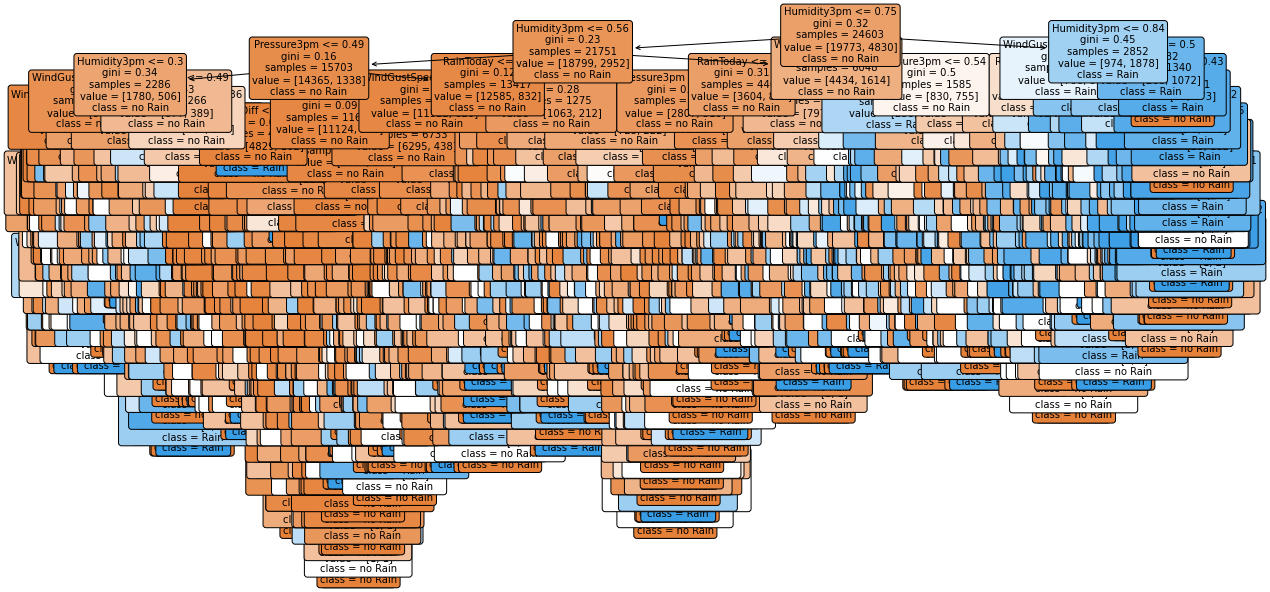
\includegraphics[width = 0.6\textwidth]{Bilder/treedefault}
	\caption{Entscheidungsbaum mit Default-Einstellungen}
	\label{fig:treedefault}
\end{figure}
Es ist leicht zu erkennen, dass dieser Baum zu viele Knoten und Blätter enthält und somit eine Überanpassung darstellt. Diese Überanpassung kann auch an dem Trainings- und Testfehler abgelesen werden. Der Trainingsfehler beträgt für den gebildeten Entscheidungsbaum 0.0005 und der Testfehler 0.2340. Der Testfehler ist damit höher als bei einem Modell, das zufällig entscheidet. Dem kann mit verschiedenen Einstellungen entgegengewirkt werden.
\subsubsection{Variationen}
%TODO: Hier fehlt noch wofür man sich entscheiden soll und warum. Bei den Einzelnen Parametern sollte glaube beschrieben werden was sie genau bewirken. Plots können hier imho raus.
Um einen übersichtlichen und brauchbaren Entscheidungsbam erzeugen zu können werden verschiedenen Einstellungen für die Parameter \emph{max\_depth, min\_ipurity\_decrease} und \emph{criterion} angewandt. Im Folgenden werden die Entscheidungsbäume dargestellt, deren Parameter mit Hilfe des \textbf{GridSearch Verfahrens} festgelegt wurden. Bei der Visualisierung liegt der Fokus auf der Struktur des Baumes und nicht darauf, dass die einzelnen Knoten identifiziert werden können.\\
\begin{figure}[H]
    \centering
     \begin{minipage}{0.30\textwidth}
        \centering
        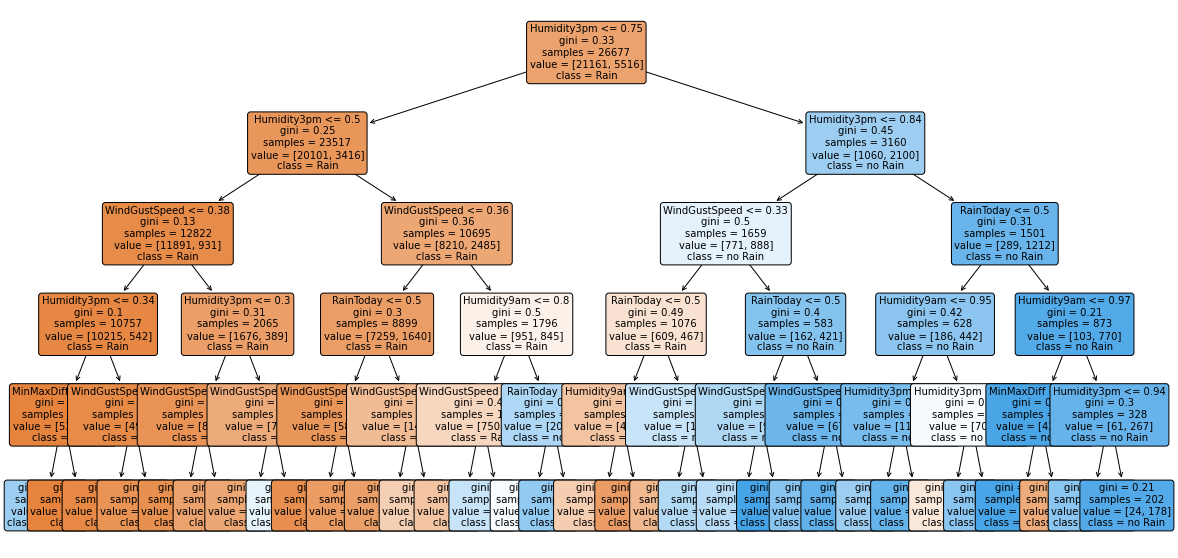
\includegraphics[width=0.9\textwidth]{Bilder/treeMaxDepth} % first figure itself
        \caption{Maximale Tiefe von 5}
        \label{fig:treeMaxDepth}
    \end{minipage}\hfill
    \begin{minipage}{0.30\textwidth}
        \centering
        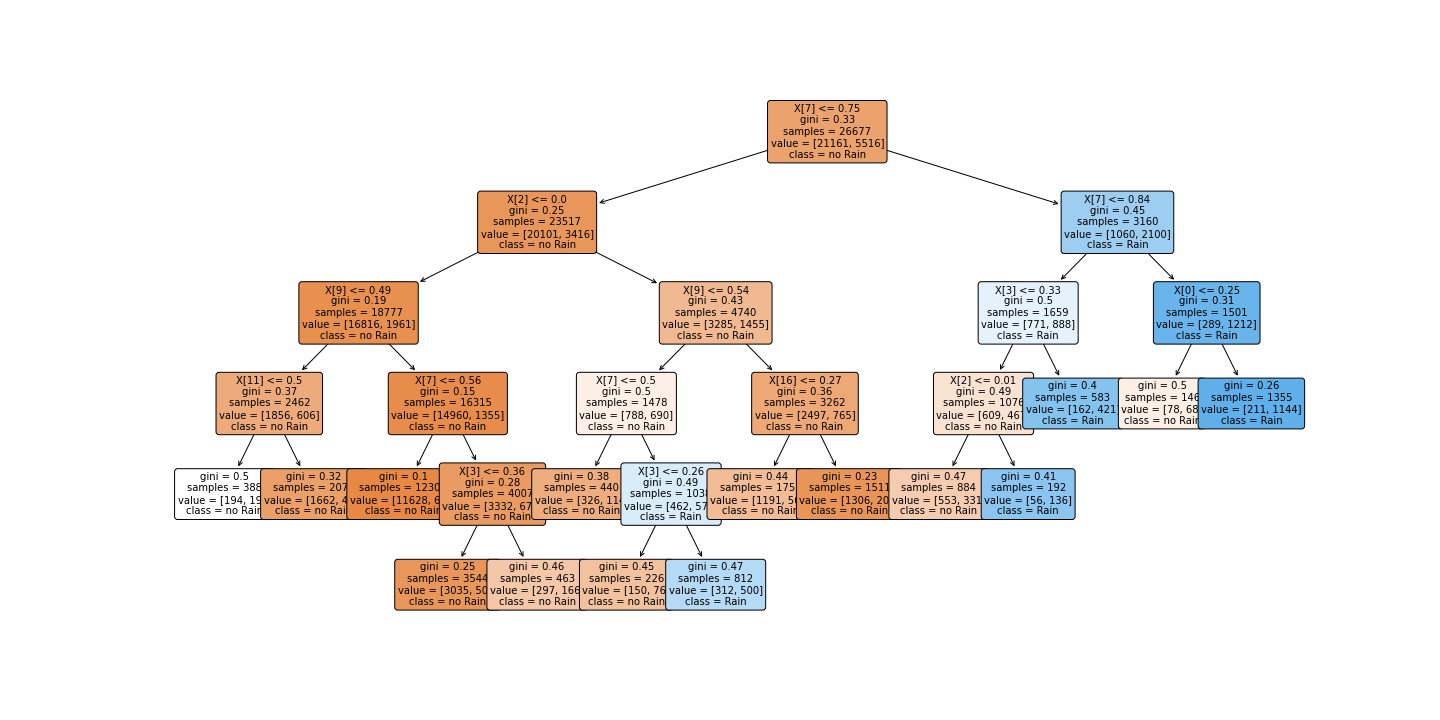
\includegraphics[width=0.9\textwidth]{Bilder/treeMinImpurityDecrease} % first figure itself
        \caption{Minimale Unschärfe Reduktion von 0.003}
        \label{fig:treeMinImpurityDecrease}
    \end{minipage}\hfill
    \begin{minipage}{0.30\textwidth}
        \centering
        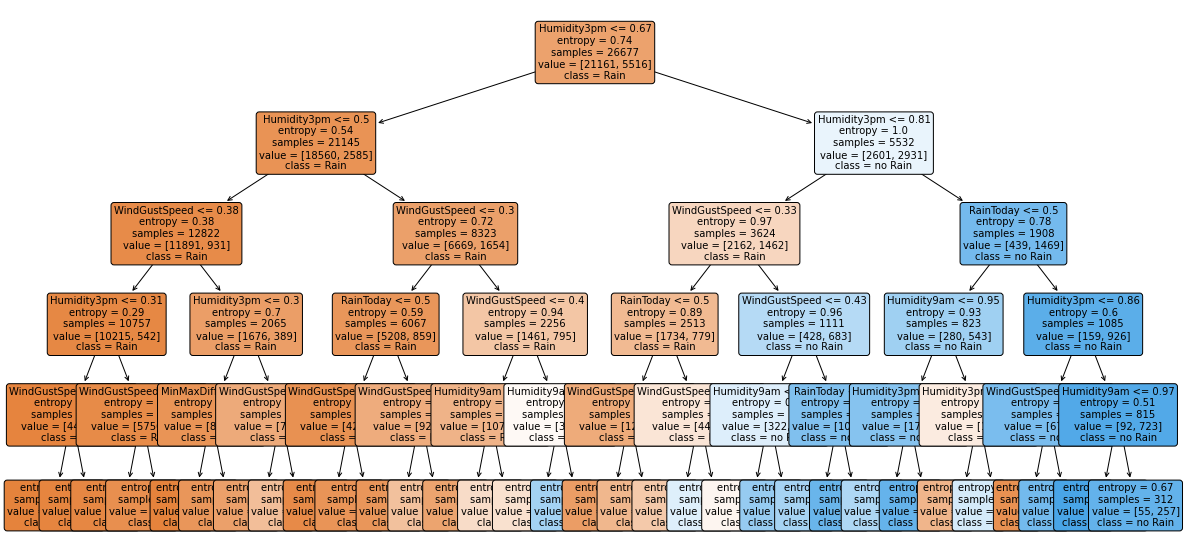
\includegraphics[width=0.9\textwidth]{Bilder/treeCriterion} % second figure itself
        \caption{Entropie als Entscheidungskriterium}
        \label{fig:treeCriterion}
    \end{minipage}
\end{figure}
\begin{description}
	\item[Maximale Tiefe]
	In Abbildung \ref{fig:treeMaxDepth} wird eine maximale Tiefe von \textbf{fünf} angegeben. Im Gegensatz zu den anderen Variationen ist dieser Baum \textbf{symmetrisch}, da jeder Ast bis zur gleichen Tiefe verfolgt wird. Dieser Baum entspricht den ersten fünf Stufen des vorher erstellten Default-Entscheidungsbaum, da der \emph{max\_depth}-Parameter den Baum einfach an der gegebenen Stufe abschneidet. % stimmt das?
	\item[Unschärfe-Reduktion] 
	In Abbildung \ref{fig:treeMinImpurityDecrease} wurde mit dem Parameter \emph{min\_impurity\_decrease} festgelegt, wie viel ein weiterer Knoten die \textbf{Unschärfe} des Entscheidungsbaumes reduzieren muss, um ausgebildet zu werden. Dabei wird jeder zu bildende Knoten einzeln bewertet, sodass es zu einem nicht symmetrischen Baum kommen kann, da nicht jeder Ast bis in die gleiche Tiefe verfolgt wird.
	\item[Entscheidungskriterium]
	In Abbildungen \ref{fig:treeCriterion} wurde zusätzlich zur maximalen Tiefe von fünf das Entscheidungskriterium angepasst. Hier wird mit Hilfe der Entropie statt des Gini-Wertes entschieden, welcher Split durchgeführt wird. Die Struktur des Baumes wird dadurch nicht geändert, jedoch können die Knoten voneinander abweichen. Die Entropie erzeugt bei sonst gleich bleibenden Parametern einen Entscheidungsbaum, der einen kleineren Testfehler aufweist.
\end{description}
%TODO Grid Search Tobi
\subsubsection{Minimal Cost-Complexity-Pruning}
Eine Möglichkeit der Vermeidung des Overfittings bietet das \emph{Cost-Complexitiy Pruning} als \emph{post-pruning} Methode. Dabei wird der voll ausgebildete Baum iterativ beschnitten, indem diejenigen Teilbäume entfernt werden, die einen festgelegten penalisierten Fehlerterm minimieren.\\
\noindent \hspace*{7mm}
Das Modul \emph{DecisionTreeClassifier} bestimmt für jeden Knoten den effektiven $\alpha$-Wert. Dabei entpricht $\alpha_{eff}$ dem $\alpha$, für das gilt: $R_{\alpha}(T_{t})=R_{\alpha}(t)$. Der Knoten mit dem geringsten effektiven $\alpha$ wird vom Baum abgeschnitten. Dieses Vorgehen wird solange wiederholt, bis der geringste effektive $\alpha$-Wert größer als der gegebenen Penalisierungs-Term \emph{ccp\_alpha} ist.\\
\noindent \hspace*{7mm}
Dabei ist zu beachten, dass die Bäume stärker beschnitten werden, je höher der gegebene Penalisierungs-Term ist, da dieser eine hohe Anzahl an Knoten bestraft (siehe auch \ref{app:abb_booklet_1}).\\
\noindent \hspace*{7mm}
Das Pruning hat Auswirkungen auf die Modellgüte, indem es die Anpassung an die Trainingsdaten reguliert. Wird der Penalisierungs-Term zu hoch gesetzt, besteht die Gefahr der Unteranpassung, ein sehr niedriger Term führt zu Overfitting. In Abbildung \ref{fig:ccp_accuracyVsAlpha} ist beispielhaft für einen Entscheidungsbaum mit Default-Einstellungen die Trainings- und Testgenauigkeit (Accuracy) für verschiedene Pruning-Parameter $\alpha$ dargestellt.
\begin{figure}[h]
	\centering
	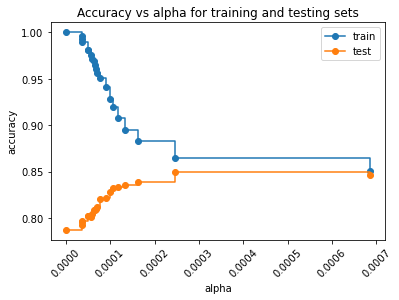
\includegraphics[width = 0.5\textwidth]{Bilder/ccp_accuracyVsAlpha.png}
	\caption{Trainings- und Testfehler für verschiedene $\alpha$-Werte}
	\label{fig:ccp_accuracyVsAlpha}
\end{figure}



